%%%%%%%%%%%%%%%%%%%%%%%%%%%%%%%%%%%%%%%%%
% Imperial College London Poster (Landscape)
% LaTeX Template
% Version 1.0 (February 22, 2024)
%
% For current versions and to report
% issues, please see:
% https://github.com/ImperialCollegeLondon/imperial_latex_templates
%
%!TEX program = xelatex
% Note: this template must be compiled with XeLaTeX rather than PDFLaTeX
% due to the custom fonts used. The line above should ensure this happens
% automatically, but if it doesn't, your LaTeX editor should have a simple toggle
% to switch to using XeLaTeX.
%
% © Imperial College London, 2024. This template, including logo and fonts, is 
% for use of Imperial staff and students only for university business. All rights 
% reserved to the copyright owners.
%
%%%%%%%%%%%%%%%%%%%%%%%%%%%%%%%%%%%%%%%%%

%----------------------------------------------------------------------------------------
%	CLASS, PACKAGES AND OTHER DOCUMENT CONFIGURATIONS
%----------------------------------------------------------------------------------------

\documentclass[
	landscape, % Landscape page orientation
	%print, % Uncomment to convert colors to CMYK for printing purposes
	%a1papersize, % Uncomment to use an A1 paper size instead of the default A0 paper size
]{ImperialPoster}

% package
\usepackage{alltt}
\usepackage{amsfonts}
\usepackage{amsmath}
\usepackage{hyphenat}
\usepackage{amssymb}
\usepackage{amsthm}
\usepackage{bm}
\usepackage{booktabs}
\usepackage{caption}
\usepackage{color}
% \usepackage[colorlinks]{hyperref}
\usepackage{enumitem}
\usepackage{etoolbox}
\usepackage{fancyhdr}
\usepackage{flafter}
\usepackage{geometry}
\usepackage{graphicx}
\usepackage{mathalfa}
\usepackage{mathdots}
\usepackage{mathrsfs}
\usepackage{mathtools}
% \usepackage{microtype}
\usepackage{multirow}
\usepackage{multicol}
\usepackage{pdflscape}
\usepackage{pgffor}
\usepackage{pgfplots}
\usepackage{siunitx}
\usepackage{slashed}
\usepackage{subfigure}
\usepackage{tabularx}
\usepackage{tikz}
\usepackage{tkz-euclide}
\usepackage[normalem]{ulem}
\usepackage{xcolor}
\usepackage{xparse}
\usepackage{xpatch}
\usepackage[all]{xy}
\usepackage{imakeidx}
\usepackage[most]{tcolorbox}

% --- Custom Color Definitions ---
% These closely match the green tones in your image
\definecolor{posterBorderGreen}{RGB}{91, 131, 80}      % Darker green for borders and text
\definecolor{posterHeaderBg}{RGB}{216, 235, 200}     % Light green background for the header

% --- Custom Environment Definition ---
\newtcolorbox{hyperbolicbox}[1]{
    enhanced,
    colback=white,                           % White body background
    colframe=posterBorderGreen,              % Outer container border color
    boxrule=3pt,                             % Border line thickness
    arc=6pt,                                 % Rounded corner radius
    boxsep=10pt,                             % Padding inside the main container
    top=5pt, bottom=10pt, left=10pt, right=10pt,
    halign=flush left,
    breakable,
    % This handles the embedded, full-width header block at the top
    before upper={
        \begin{tcolorbox}[
            colback=posterHeaderBg,
            colframe=posterBorderGreen,
            boxrule=1.5pt,
            arc=4pt,
            width=\linewidth,
            top=8pt, bottom=8pt, left=10pt, right=10pt,
        ]
        \centering{\color{posterBorderGreen}\sffamily\bfseries\large #1}
        \end{tcolorbox}
    }
}




\theoremstyle{definition}
\newtheorem{thm}{Theorem}
\newtheorem{defi}[thm]{Definition}

\newcommand{\C}{\mathbb{C}}
\newcommand{\R}{\mathbb{R}}
\newcommand{\Q}{\mathbb{Q}}
\newcommand{\Z}{\mathbb{Z}}
\newcommand{\N}{\mathbb{N}}
\renewcommand{\H}{\mathbb{H}}
\newcommand{\F}{\mathbb{F}}

\newcommand{\topo}{\mathcal{T}}
\newcommand{\B}{\mathcal{B}}
\renewcommand{\S}{\mathcal{S}}
% Symbols
\newcommand{\noteq}{\not=}
\newcommand{\re}{\mathrm{Re\,}}
\newcommand{\im}{\mathrm{Im\,}}
\newcommand{\nexist}{\not\!\exists\,}
\newcommand{\abs}[1]{\left\lvert #1\right\rvert}
\newcommand{\norm}[1]{\left\lVert #1\right\rVert}
\newcommand{\floor}[1]{\left\lfloor #1\right\rfloor}
\newcommand{\ceil}[1]{\left\lceil #1\right\rceil}
\newcommand{\set}[1]{\left\{#1\right\}}
\newcommand{\closure}[2][3]{%
{}\mkern#1mu\overline{\mkern-#1mu#2}}
\newcommand{\interior}{\mathrm{Int\,}}
\newcommand{\upint}{\mathchoice%
    {\mkern13mu\overline{\vphantom{\intop}\mkern7mu}\mkern-20mu}%
    {\mkern7mu\overline{\vphantom{\intop}\mkern7mu}\mkern-14mu}%
    {\mkern7mu\overline{\vphantom{\intop}\mkern7mu}\mkern-14mu}%
    {\mkern7mu\overline{\vphantom{\intop}\mkern7mu}\mkern-14mu}%
  \int}
\newcommand{\lowint}{\mkern3mu\underline{\vphantom{\intop}\mkern7mu}\mkern-10mu%
\int}
\newcommand{\aand}{\quad\text{and}\quad}
\newcommand{\res}[1]{\!\mid_{#1}}
\newcommand{\normal}{\unlhd}
\newcommand{\group}[1]{\langle#1\rangle}
\renewcommand{\tt}[1]{\quad\text{#1}\quad}
\renewcommand{\d}{\mathop{}\!\mathrm{d}} 
\renewcommand{\emptyset}{\varnothing}
\DeclareMathOperator{\lcm}{lcm}
\DeclareMathOperator{\diam}{diam}
\DeclareMathOperator{\id}{id}
\DeclareMathOperator{\Bd}{Bd}
%----------------------------------------------------------------------------------------
%	POSTER INFORMATION
%----------------------------------------------------------------------------------------

\postertitle{\LARGE On the connection between the action of $\operatorname{PSL}(2,\Z)$ on $\H$ and the classification of lattices $\Lambda\subset\C$} % The poster title, can be split across multiple lines manually with \\

% Contributor/author names, can be split across multiple lines manually with \\
% % Add affiliations using the \affiliation{} command
% \posterauthors{Name of contributor\affiliation{1, 2},\\ Name of contributor\affiliation{1},\\ Name of contributor\affiliation{3}}

% Command to output coauthor logos to the right of the Imperial logo in the header of the poster
% % If no coauthor logos are required, remove or comment out this command
% \coauthorlogos{
% 	\coauthorlogo[4cm]{Grey_16-9.pdf} % Use the optional parameter to specify a height for the logo
% 	\coauthorlogo[4cm]{Grey_16-9.pdf} % Use the optional parameter to specify a height for the logo
% 	\coauthorlogo{Grey_16-9.pdf} % Not specifying the optional parameter will make the logo the same height as the Imperial logo
% }

%----------------------------------------------------------------------------------------

\begin{document}

%----------------------------------------------------------------------------------------
%	EXAMPLE POSTER LAYOUT 1
%----------------------------------------------------------------------------------------

\titlesection % Output the title section, automatically populated using the information in the POSTER INFORMATION block above

\medskip % Vertical whitespace


\begin{multicols}{4}

    \begin{hyperbolicbox}{The action of $\operatorname{PSL}(2,\Z)$ on $\H$}
        \small

        \begin{defi}
            Let $\H$ denote the upper half of the complex plane:
            $$
            \H=\set{z\in\C:\Im z>0}
            $$
            Let $\operatorname{SL}(2,\Z)$ denote the group of matrices of $\Z^{2\times 2}$ with determinant $1$. We define $\operatorname{PSL}(2,\Z)=\operatorname{SL}(2,\Z)/\set{\pm I}$. For each $M=\begin{pmatrix}
                a&b\\c&d
            \end{pmatrix}\in\operatorname{PSL}(2,\Z)$, it acts on $\H$ via the corresponding M\"obius map:
            $$
            z\mapsto\frac{az+b}{cz+d}
            $$
        \end{defi}

        \begin{thm}
            $\operatorname{PSL}(2,\Z)$ is generated by the M\"obius maps $z\mapsto z+1$ and $z\mapsto-1/z$.
        \end{thm}
        \begin{proof}
            Let
            $$
            T=\begin{pmatrix}
                1&1\\0&1
            \end{pmatrix}\aand
            S=\begin{pmatrix}
                0&-1\\1&0
            \end{pmatrix}
            $$
            be the matrices corresponding to $z\mapsto z+1$ and $z\mapsto-1/z$, respectively.
            
            For any matrix $M=\begin{pmatrix}
                a&b\\c&d
            \end{pmatrix}\in\operatorname{PSL}(2,\Z)$. If $\abs{a}\geq\abs{c}>0$, there exists unique $k,r\in\Z$ such that $a=kc+r$ where $0\leq r<\abs{c}\leq\abs{a}$. It follows that 
            $$
            \begin{pmatrix}
                a&b\\c&d
            \end{pmatrix}=
            T^k\begin{pmatrix}
                r&b-kd\\c&d
            \end{pmatrix}
            $$
            If $\abs{c}>\abs{a}>0$, there exists unique $k,r\in\Z$ such that $c=ka+r$ where $0\leq r<\abs{a}$. It follows that
            $$
            \begin{pmatrix}
                a&b\\c&d
            \end{pmatrix}=
            S\begin{pmatrix}
                c&d\\-a&-b
            \end{pmatrix}=
            ST^{-k}\begin{pmatrix}
                r&d-kb\\-a&-b
            \end{pmatrix}
            $$
            Repeatedly apply the two steps above, which will terminate in a finite number of times since $\abs{a}$ decreases each time. $M$ then equals a combination of $T,S$ and a matrix with $a=0$ or $c=0$, which is obviously generated by $T$ and $S$. We conclude that $M\in\group{T,S}$ and then $\group{T,S}=\operatorname{PSL}(2,\Z)$.
        \end{proof}

        \begin{defi}
            By a \textit{fundamental domain} for $\H/\operatorname{PSL}(2,\Z)$ we mean an open subset $\mathcal{F}\subset\H$ where $\mathcal{F}\cap\gamma\mathcal{F}=\emptyset$ for $\gamma\in\operatorname{PSL}(2,\Z)\setminus\set{I}$ and $\bigcup\gamma\closure{F}=\H$.\cite{milneMF}
        \end{defi}
        \vspace{-1em}
        
        Figures below visualize the action of $\operatorname{PSL}(2,\Z)$ on $\H$ and the standard fundamental domain $\mathcal{F}$ (shaded area) given by

        $$
        \mathcal{F}=\set{z\in H:\abs{\Re z}<\frac{1}{2},\abs{z}> 1}
        $$  
        
        \begin{figure}[H]
            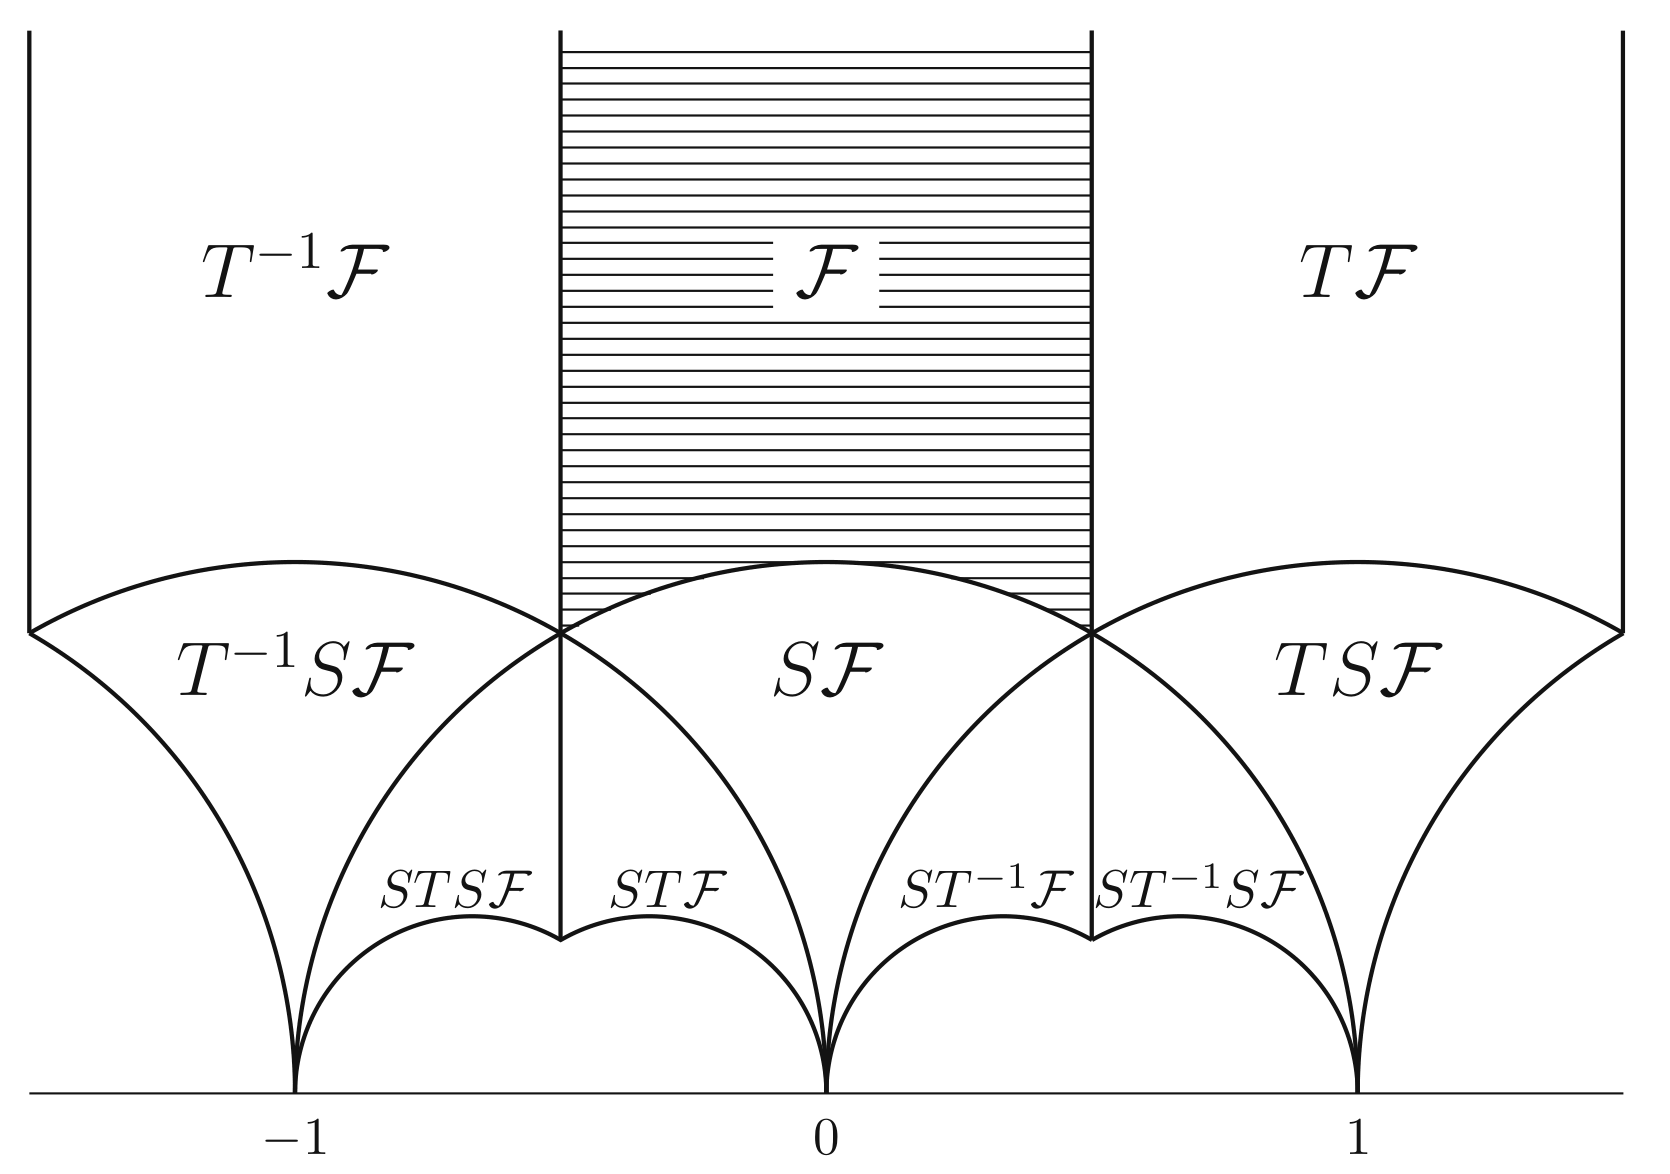
\includegraphics[width=0.4\linewidth]{Images/fund1.png}
            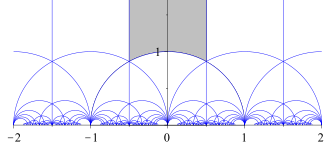
\includegraphics[width=0.55\linewidth]{Images/fund2.png}
        \end{figure}
        
        Each hyperbolic triangle in the images can be translated from the fundamental domain via a M\"obius map in $\operatorname{PSL}(2,\Z)$.
    \end{hyperbolicbox}
        
    % \columnbreak

    \begin{hyperbolicbox}{Lattices $\Lambda\subset\C$}
    \small
    \begin{defi}
        A \textit{lattice} $\Lambda$ in the complex plane is an additive discrete subgroup of $\C$. \cite{LozanoEC}
        Equivalently, $\Lambda\subset\C$ is a lattice if there are $p,q\in\C$ linearly independent over $\R$, i.e. $\frac{p}{q}\notin\R$, such that
        $$
        \Lambda=\group{p,q}=\set{ap+bq:a,b\in\Z}
        $$
    \end{defi}
    As an example, the figure below shows the lattice $\group{\frac{1}{2}+\frac{3}{2}i,\frac{3}{2}+\frac{3}{2}i}$.
    \begin{figure}[H]
        \centering
        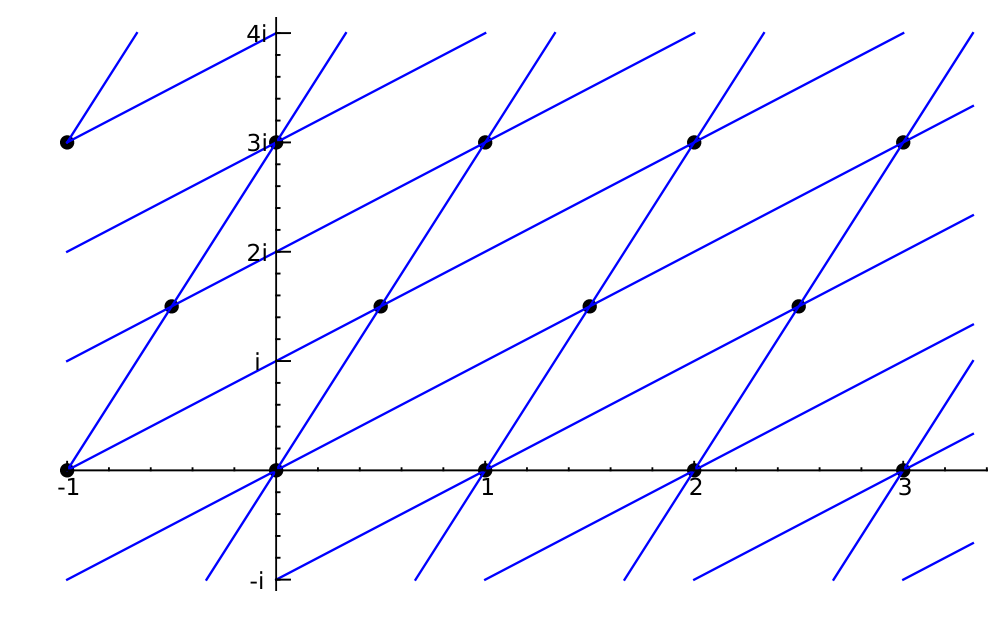
\includegraphics[width=0.5\linewidth]{Images/lat1.png}
    \end{figure}
    For a lattice $\Lambda=\group{p,q}$, one can prove that the parallelogram
    $$
    \mathcal{F}=\set{ap+bq:0\leq a,b<1}
    $$
    is a fundamental domain for $\C/\Lambda$.
    \begin{thm}\cite{LozanoEC}\label{thm5}
        Let $\Lambda=\group{p,q}$ and $\Lambda'=\group{p',q'}$ be two lattices with $\frac{p}{q},\frac{p'}{q'}\in\H$. We have $\Lambda=\Lambda'$ if and only if there is a matrix $M\in\operatorname{SL}(2,\Z)$ such that 
        $$
        \begin{pmatrix}
            p'\\q'
        \end{pmatrix}=M
        \begin{pmatrix}
            p\\q
        \end{pmatrix}
        $$
    \end{thm}
\end{hyperbolicbox}
    
	% \columnbreak

    \begin{hyperbolicbox}{Homothetic lattices}
    \small
    We want to regard two lattices to be `similar' if one can be converted to the other via some basic geometric transformations which preserves most of the properties of the lattice structure. Under this idea, we give the following definition.

    \begin{defi}
        Two lattices $\Lambda$ and $\Lambda'$ are said to be \textit{homothetic} if there is $c\in\C\setminus\set{0}$ such that $\Lambda'=c\Lambda$. \cite{milneMF}
    \end{defi}
    
    It's easy to see that, if $\Lambda'=re^{i\theta}\Lambda$ are homothetic, then $\Lambda$ can be transformed to $\Lambda'$ via a dilation by $r$ and a rotation by $\theta$.

    For the structure-preserving property, one has the following theorem.

    \begin{thm}
        Let $\Lambda$ and $\Lambda'$ be two lattices in $\C$. Then $\C/\Lambda$ is isomorphic to $\C/\Lambda'$ if and only if $\Lambda$ and $\Lambda'$ are homothetic. \cite{silvermanTA}
    \end{thm}
\end{hyperbolicbox}

    % \columnbreak

    \begin{hyperbolicbox}{Normalization of lattices}
    \small
    \begin{defi}
        Since we only care about $\Lambda$ up to homothety, for a lattice $\group{p,q}$ with $\tau=\frac{p}{q}\in\H$, we can normalize it to a homothetic lattice $\Lambda_{\tau}=\group{\tau,1}=\frac{1}{q}\group{p,q}$. \cite{silvermanAT} 
    \end{defi}
    
    However, there might also be homothetic normalized lattices such as $\group{i,1}=\group{i+1,1}$. We identify them using the following theorem.

    \begin{thm}
        Let $\tau,\tau'\in\H$. $\Lambda_\tau$ and $\Lambda_{\tau'}$ are homothetic if and only if $\tau$ and $\tau'$ are related with a M\"obius map $\tau'=\frac{a\tau+b}{c\tau+d}$ where $\begin{pmatrix}
            a&b\\c&d
        \end{pmatrix}\in\operatorname{PSL}(2,\Z)$.
    \end{thm}
    \begin{proof}
        By definition, $\Lambda_\tau$ and $\Lambda_{\tau'}$ are homothetic if and only if there is $z\in\C\setminus\set{0}$ such that $\Lambda_{\tau'}=z\Lambda_\tau$, which is equivalent to
        $$
        \group{\tau',1}=\group{z\tau,z}
        $$
        which by \hyperref[thm5]{Theorem 5} holds if and only if there is $\begin{pmatrix}
            a&b\\c&d
        \end{pmatrix}\in\operatorname{SL}(2,\Z)$ such that
        $$
        \begin{pmatrix}
            \tau'\\1
        \end{pmatrix}=\begin{pmatrix}
            a&b\\c&d
        \end{pmatrix}\begin{pmatrix}
            z\tau\\z
        \end{pmatrix}\iff \tau'=\frac{a\tau+b}{c\tau+d}
        $$
    \end{proof}

    This theorem points out the relationship between the action of $\operatorname{PSL}(2,\Z)$ on $\H$ and the classification of $\Lambda\subset\C$.
    
    Specifically, if we use $\mathcal{L}$ to denote the set of all lattices in $\C$, and define an equivalence relation $\sim$ on $L$ by $\Lambda\sim\Lambda'$ if and only if $\Lambda$ and $\Lambda'$ are homothetic, then there is a bijection from $\H/\operatorname{PSL}(2,\Z)$ to $\mathcal{L}/\sim$ given by
    $$
        f:\tau\mapsto\Lambda_\tau
    $$
\end{hyperbolicbox}

    \begin{hyperbolicbox}{$j$-invariant}
    \small
    \begin{defi}
        The $j$-invariant is a function from $\H$ to $\C$ defined by
        $$
        j(\tau)=1728\frac{g_2(\tau)^3}{\Delta(\tau)}
        $$
        The core property of the function is that $j(\tau)=j(\tau')$ if and only if there is a M\"obius map in $\operatorname{PSL}(2,\Z)$ such that $\tau'=\frac{a\tau+b}{c\tau+d}$, or equivalently, $\Lambda_\tau$ is homothetic to $\Lambda_{\tau'}$ \cite{silvermanAT}. Therefore, $j$-invariant acts as an isomorphism from $\H/\operatorname{PSL}(2,\Z)$ to $\C$. On the other hand, when we apply the correspondence between $\H/\operatorname{PSL}(2,\Z)$ and $\mathcal{L}/\sim$ we just deduced into the $j$-invariant, we can, in fact, view it as a parameterization of each equivalence class to points of $\C$.   
    \end{defi}
\end{hyperbolicbox}

    \begin{hyperbolicbox}{Summary}
    In this poster, we explored the action $\operatorname{PSL}(2,\Z)$ on $\H$. We observed that the action of $\operatorname{PSL}(2,\Z)$ tessellates $\H$ into copies of a fundamental domain, where any two triangles can be associated by a M\"obius map in $\operatorname{PSL}(2,\Z)$.

    Then we studied the lattice structure in $\C$: any lattice is generated by independent $p,q\in\C$. While homothety provides a notion of similarity among lattices, it actually generates an equivalence relation, based on which one can classify all complex lattices.

    We finally discovered that $\Lambda_\tau$ is homothetic to $\Lambda_{\tau'}$ if and only if $\tau'$ can be transformed from $\tau$ via a M\"obius map in $\operatorname{PSL}(2,\Z)$. It follows that the orbit space $\H/\operatorname{PSL}(2,\Z)$ and the set of lattices up to homothety have the same structure and are connected by a bijection $\tau\mapsto\Lambda_\tau$. The $j$-invariant, as a parameterization of equivalence classes, gives us an algebraic view of this connection.
\end{hyperbolicbox}
    
    \begin{hyperbolicbox}{References}
    \begingroup\patchcmd{\thebibliography}{\section*{\refname}}{}{}{}
    \vspace{-1em}
    \begin{thebibliography}{9}
    \normalsize
    \bibitem{milneMF}
    J.~S. Milne (2017) \textit{Modular Functions and Modular Forms (v1.31)}, www.jmilne.org/math.
    
    \bibitem{LozanoEC}
    Lozano-Robledo, Álvaro (2011) \textit{Elliptic Curves, Modular Forms and their L-functions}. https://doi.org/10.1090/stml/058 
    
    \bibitem{silvermanAT}
    Silverman, J.H. (1994) \textit{Advanced Topics in the Arithmetic of Elliptic Curves}. https://doi.org/10.1007/978-1-4612-0851-8

    \bibitem{silvermanTA}
    Silverman, J. H. (2009). \textit{The Arithmetic of Elliptic Curves}. https://doi.org/10.1007/978-0-387-09494-6
    
    \end{thebibliography}
    \endgroup
\end{hyperbolicbox}
    
\end{multicols}

\end{document}
